\chapter{Case study : RescueME SPL}
\label{ch:caseStudy}

\begin{quotation}[ The Experience of Insight]{Joseph Goldstein}
If we're facing in the right direction, all we have to do is keep on walking.
\end{quotation}



\section{ Introduction }
\label{sc:experimentIntroduction}

In this chapter, will be described a case study where the \ac{SPLICE} tool was tested during a real \ac{SPL} development. The study was conducted inside a research laboratory and included the migration from a manual Software Engineering process to the \ac{SPLICE} tool and the proposed metamodel. To validate the tool, we proposed some research questions and conducted a survey. 

This Chapter is organized as follows: \secref{sc:definition} defines this case study; in \secref{sc:researchMethod} the planning of the case study takes place; \secref{sc:datacollection} shows the analysis and interpretation of the results; \secref{sc:threats} analyses the possible threats  to  validity of our study; \secref{sc:leassonsLearned} describes the lessons learned during this study; and \secref{sc:expsummary} presents the findings and summarizes this chapter.

\section{ Definition }
\label{sc:definition}

\subsection{Context}
During the months of June and November 2013, we performed a case study in the “National Institute of Software Engineering (I.N.E.S)”, a Software Engineering research laboratory, composed of 11 Ph.D. candidates. The laboratory developed a \ac{SPL} called RescueMe, which was built following a \ac{SPL} agile process. 
The RescueMe is a product line developed in Objective-C for iOS devices. RescueMe is designed to to help its users in dangerous situations. The start screen of the application consists of a button that when pressed send messages to the user contacts asking for help. RescueMe get the contacts from the phone address book or from social networks, such as Facebook and Twitter, depending on the used version.

\begin{figure}[htp]
\begin{center}
  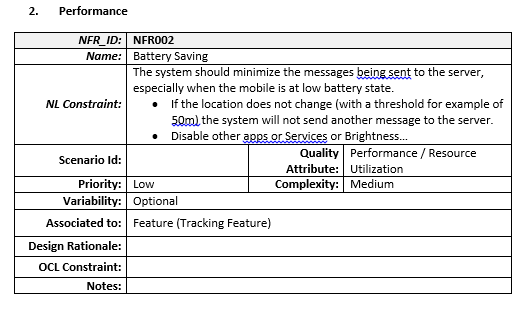
\includegraphics[width=10cm]{chapters/experiment/img/old-req.PNG}
  \caption[Product Development]{Older non-functional requirement}
  \label{fg:spl-reqdoc}
\end{center}
\end{figure}

RescueMe had an iterative and incremental development, carried out by four developers, with a face-to-face meeting at the end of each sprint. These meetings were responsible for evaluating results, and planing the next sprint. The group manually maintained the \ac{SPL} process based on a set of external tools. Before using \ac{SPLICE}, they used the SourceForge\footnote{http://www.sourceforge.net} service for issue tracking and \acf{VCS}. All the requirements artifacts where maintained using text documents questionnaires, as can be seen on \figref{fg:spl-reqdoc}.
The \ac{SPLICE} was introduced to manage the \ac{SPL} process and all artifacts were migrated to it. After the migration, the development continued to use only the \ac{SPLICE} to manage the application lifecycle.

\subsection{Research Questions}

The \ac{SPLICE} is a complete environment for Software Product Lines development, and many aspects can be analyzed. However, in this work the main objective is to analyze the effectiveness of the traceability through integration of the technologies on the tool, and how the tool influences the \acf{SPL} lifecycle. 
In order to evaluate these aspects in our proposal, we defined three case study research questions:

\begin{itemize}
\item \textbf{From the stakeholder perspective, how the traceability is solved with the \ac{SPLICE}?}

Rationale: The goal is to verify if the tool can provide traceability support, and from the stakeholder perspective, how it was solved.

\item \textbf{How positively the tool improved the application lifecycle?}

Rationale: The tool manages the whole process, and this question verifies if the outcome is positive.
\item \textbf{How negatively the tool impacted the application lifecycle?}

Rationale: In this question, the stakeholder evaluates how negatively the \ac{SPLICE} interfered with the process.
\end{itemize}



\section{Data collection}
\label{sc:researchMethod}

In this case tudy, we selected surveys as a data collection instrument. Survey  is  a  data-gathering  mechanism  in  which participants answers  questions  or  statements  previously developed and according to \cite{Kitchenham2008} , they are probably  the  most  commonly used instrument to gather opinions from experts. Expert Surveys is a kind of study conducted through a research  applied  to  people  who  are  considered  experts  in  a  field,  in  order  to  identify speculations,  guesses  and  estimates,  which  may  serve  as  a  cognitive  input  in  some decision process \citep{Chhibber1992} 


The survey design is based on \cite{Kitchenham2008} guidelines and is composed of a set of personal questions, closed-ended and open-ended questions related to the research questions. The remain of this section contains the overall process applied in this study and the methodology.

\subsection{Survey Design}

In  this  survey,  we  used  the  cross-sectional  design,  which  participants  were  asked  about  their  past  experiences  at  a  particular  fixed point in time. This survey was performed as a self-administered printed questionnaire. We  collected  all  data  for  analysis in January, 2014.  

\subsection{Developing the Survey Instrument}

The  questionnaire,  which  composes  the survey,  was  defined  based  on  the  steps  defined  in \cite{Kitchenham2008} , and although they suggest the  use  of  closed  questions  in  self-administered  questionnaires,  our question was composed of closed questions with an open field to justification,  as the tool usage is something very subjective and we wanted to capture  the  researcher  opinion. The questionnaire was composed of three personal questions, eight  closed questions with justification fields, and three open questions. The closed questions were formulated to measure and quality the data, while getting personal feedback. The open questions were built to collect the experts’ experiences and the impressions about the tool.


\subsection{Evaluating the Survey Instrument}



After defining the questions for our survey, it is necessary to evaluate it, in order to check whether is enough to address the preliminary stated goals. Evaluation is often called pre-testing and according to \cite{Kitchenham2008} has several different goals :

\begin{itemize}
\item To check that the questions are understandable.
\item To  assess  the  likely  response  rate  and  the  effectiveness  of  the  follow-up procedures.
\item To evaluate the reliability and validity of the instrument.
\item To ensure that our data analysis techniques match our expected responses.
\end{itemize}


We validated the  questionnaire  by  asking Software  Engineering researchers from the RiSE research group to analyze and suggest modifications. The suggestions where discussed and the questionnaire modified accordingly.  It is important to reinforce that the authors were not considered during the pilot test. The questionnaire can be seen in the Appendix 1.



\subsection{Expert Opinion}

An  important  step  on expert opinion   survey  is  looking  for  expert  judgments,  since  an  expert  is  a knowledgeable authority on the research domain  [Chhibber et al., 1992].  Considering this, the subjects should be chosen based on the most relevant expertise, most accurate estimates or judgments. Our selection criteria was: The expert should have a considerable knowledge demonstrated through academic experience or Industry experience. They also must have a strong background in Software engineering and more specifically in \acf{SPL}. Another very important and limiting criteria is that the expect should have availability to use the tool and be involved with the specific analyzed case study , the RescueME.

We did not use any sampling method as suggested by \cite{Kitchenham2008}, because the target population was already very small. At the beginning, we selected four SPL experts, as potential candidates. However, one of them did not receive the invitation emails, and another did not answer our invitation. Thus, we had two experts that participated in this survey.  

The experts who answered the questionnaire are  showed in Table  \ref{table:expertsselected},  all the experts have more than 5 years of experience in Software Engineering, and more than 4 years on \ac{SPL} specifically . The purpose of this table is to show that the \ac{SPL} experts are people that have been involved in the SPL community, and their names are showed in order to increase the confidence of our research.

\begin{table}
\begin{center}
\centering
\small
\tabcolsep=0.11cm
    \begin{tabular}{|l|l|l|l|}
    \hline
    Name             & Occupation      & SE experience & SPL experience                     \\ \hline
    Raphael Oliveira & Ph.D. candidate & 10 years                        & 6 years                                               \\ \hline
    Tassio Vale      & Ph.D. candidate & 6 years                         & 4 years, on academic and industrial projects. \\ \hline
    \end{tabular}
        \caption {Experts Selected}
        \label{table:expertsselected}
        \end{center}

\end{table}

\subsection{Analyzing the data}

In  order  to  collect  the  data, the  experts  filled a printed questionnaire.  From the  three  invited  researchers  only  two  reported  their  answers. 
After designing and running the survey, the next step was to analyze the collected data. The main analysis procedure was to check all responses, tabulate the data, identify the findings and classify the options. 

\section{Results}
\label{sc:datacollection}

In  this  section  the  analysis  of  the  collected  data  are  presented, discussing  the  given  answer  for  each  question. Three of the fourteen questions were personal questions such as name and experience and where already reveled on the previous section.

\subsubsection{Tool usage difficulties}
Considering the question \textbf{There was any difficult during the execution of some activity in the tool ?},  one expert declared in that did not found any problem using the tool, however another subject indicated that \textit{“The SPLICE assets management should be the initial screen”}. Actually the initial screen is the \textit{Wiki}.

\subsubsection {Tool interference in workflow}
In the question:  \textbf{How the usage of the tool altered your workflow? }, one expert pointed that the tool did not altered his workflow, since the tool \textit{“offered the option to specify the needed asserts during the SPL lifecycle.”}, interestingly another expect pointed the exactly opposite and complained that \textit{“The tool should provide a way to customize the necessary assets for each project, so it can be used in several SPL projects”}.


\subsubsection{Assets creation difficulties}
Considering the question \textbf{Did you have any problems creating assets ?} , 
All respondents pointed that they had no problems during the assets creation.

\subsubsection{Blame changes}
Considering the question \textbf{ Did the tool gave you enough information to identify who did a specific modification in an asset ?} , both experts declared that this information was clearly presented and complete.

\subsubsection{Traceability}

In the question \textbf{Do you consider that tool aided the traceability among the assets?} all experts replied \textit{“Yes”}. We asked for justification and one said that \textit{“The tool deals in an easy way with the traceability among assets. For example, it is easy to check what products have a determinate Feature, since there is a field in the feature details that shows this information (Products with this Feature)”}.
Another respondent stated that (the tool) \textit{“...provides links for different types of assets to be related in the tool, and it provides, for instance, the ability to analyze the impact of changes”}. From the answer of the respondents, we could assume that the tool did address the traceability problem, providing a level of traceability to the managed assets.


\subsubsection{Expected traceability links}
All respondents indicated in the question \textbf{Did you expect any traceability link not available in the tool? If so, which one(s) ?} , that they did not expected any other traceability link, from what is offered by the tool.

\subsubsection{Traceability links navigation}
Considering the question \textbf{ What is your opinions on navigating among traceability links ?}, one expert pointed that the Traceability links navigation in \ac{SPLICE} was intuitive and \textit{“…simple because each traceability link has the ‘asset name’ on the defined value (i.e. compile time) that lead to more details of the ‘’asset’ or ‘define value’ when clicked”}. 

However, another expert replied that \textit{“The traceability links make software engineers to think the assets as part of a unique SPL. When these links are not available, the assets seems disconnected and I can’t have an overall view of the SPL inconsistencies it might cause when specifying new assets.”}. This question have a problem, as it should state more clearly that we want to know about the options on navigating among traceability links using the \ac{SPLICE} tool. We do not know if he is complaining about the tool, or traceability navigation in general. We do not think that is directly related to the too because in a previous question he declared that no traceability link was missing in the \ac{SPLICE}.


\subsubsection{Reporting}
In the  question \textbf{ In your opinion, the reports generated were satisfactory ?} , one respondent fully agreed that the generated reports were satisfactory. Conversely, another respondent stated that is missing the \textit{“The analysis of impact for changes in the SPL assets. Based on an asset that is changed, I can visualize the impacted assets and the effort to make modification in the SPL”}. The \ac{SPLICE} do have impact change analysis, but just for assets deletion, this is a point that can be improved.


\subsubsection{Tool Helpfulness}
Considering the question \textbf{Do you think that the proposed tool would aid you during a SPL process ? Would you spontaneously use the tool hereafter? }, all experts fully agreed that the tool was helpful and they would use in another project. One expert even stated that \textit{“One of the biggest problems within SPL documentation when performed in spreadsheets or documents files is to keep updated the traceability information among the SPL assets after evolving them. The proposed tool helps in dealing with this problem”}.


\subsubsection{Positive points}
We asked the experts the question \textbf{What are the positive points of using the tool? } , and the positive points of the tool according to them are:
\begin{itemize}
\item Traceability among assets.
\item Version control system.
\item Change history.
\item Report generation.
\item Integration with variability mechanisms.
\item Integration of different software engineering support tools.
\item Feature oriented approach.
\end{itemize}
Most of them mentioned positive points are functional requirements of the tool, which could demonstrate that some of our objectives was been fulfilled by the \ac{SPLICE}.

\subsubsection{Negative points}
In Contrast with the previous question, we also asked \textbf{ What are the negative points of using the tool?}. Only two points were mentioned, as follow:
\begin{itemize}

\item \textbf{Pre-defined set of assets is available}. \textit{“If a SPL manager decides to include a new asset, a new version of the tool must be deployed”}.

\item \textbf{No variability mechanisms in source code}. \textit{“The integration with variability mechanisms in source code is not available. Then, the derivation is not complete”}.
\end{itemize}


\subsubsection{Suggestions}
As a final point, we asked \textbf{Please, write down any suggestion you think might be useful}.
One expert suggested to \textit{“Turn the tool flexible to include or remove assets for a specific project”}. The other expert suggest that \textit{“The analysis of change impacts can be very useful. You can use the estimatives ( Story points, for example) to calculate the effort spent to change a feature, user story and so on”}. 
Although one of our non-functional requirement is to provide \textit{“Metamodel flexibility”}, we implement this on a compile time. Both suggestion has been noted to future improvement to the tool.

\section{Threats to validity}
\label{sc:threats}
There  are some  threats  to  the  validity of our  study,  which  were briefly described and discussed:


\begin{itemize}
\item Research  questions:  The  research  questions  we  defined  cannot provide  complete  coverage  of  all the features covered by the tool. We considered just some important point: traceability, advantages and disadvantages. 

\item Sample  size:  The  most  obvious  threat  to  internal  validity  is  the sample  size,  which  was very small. Fowler  (2002)  suggests  that  there  is  no  equation  to  exactly determine the sample size, but we recognize a more ample study help to generalize the case study results.

\end{itemize}

\section{Findings}
\label{sc:leassonsLearned}


Analyzing the answers, just one developer reported difficulties during the tool usage. He reported problems with the fact the initial screen is the collaborative document and not the assets screen, which is hidden behind a menu item. We will make the software more customizable in the future. No users reported difficulties creating asserts or identifying who performed modifications to assets. No major usability problem was found, and all were able to use and evaluate the tool without supervision. This can indicate that the tool fulfilled the requirements of Usability and Accountability.

All the experts explicitly declared that the tool was useful, aided on the assets traceability, provided all the traceability links they wanted and offered a valuable set of features. They also stated that would, spontaneously, use the tool in future \ac{SPL} projects. 

The experts also mentioned some points of improvement during the survey. One interesting problem vocally expressed by one expert was inability to configure the process and the metamodel. This is a non-functional requirement of the tool, and the \ac{SPLICE} architecture is very capable of it. However, this require editing some files manually, so visual editor should be added to the tool to address this problem.

Some other problems includes the need to a better change impact analysis and integration with variability in source code, to perform product line derivation. The latter future was postponed because of time limitations of an undergraduate project, and is planned for a future version.


\section{Summary}
\label{sc:expsummary}

This chapter presented the definition, planning, operation, analysis and interpretation of a case study to evaluate the \ac{SPLICE} tool. The case study was conducted inside the research laboratory “National Institute of Software Engineering (I.N.E.S)”, and a survey was administered to the experts of the laboratory.
After concluding the case study and the questionnaires, we gathered information that can be used as a guide to improve the tool, and an indicator about the actual status of the tool. The results of the experiment pointed out that the \ac{SPLICE} address the traceability problem and was considered useful to all experts. However, some points of improvements were raised, that we plan to fix on future versions. In addition, the case study design and the lessons learned were also presented.

Next chapter presents the concluding remarks and future work of this dissertation.



